\documentclass{article}
\usepackage[utf8]{inputenc}
\usepackage[T1]{fontenc}
\usepackage[russian]{babel}
\usepackage{tikz}
\usepackage{graphicx}
\usepackage{titlesec}
\usepackage{amsfonts}
\usepackage{amsmath}
\usepackage[left=2cm,right=2cm,
    top=2cm,bottom=2cm,bindingoffset=0cm]{geometry}
\renewcommand{\thesection}{\arabic{section}}
\titleformat{\section}{\large\bfseries}{\thesection}{1em}{}
\title{Пределы}
\author{Каренин Константин Витальевич}
\date{19.10.2023}
\begin{document}

\begin{titlepage}
    \centering
    \vspace*{0.5 cm}
    
    \textsc{\LARGE \textbf{Математический анализ}}
    \vspace{1.5cm}
    
    \rule{\linewidth}{0.2 mm} \\[0.4 cm]
    { \huge \bfseries Пределы}
    \rule{\linewidth}{0.2 mm} \\[1.5 cm]
    
    \Large Выполнили: \\
    Каренин Константин \\
    Темиров Тимур \\
    Гонин Сергей \\
    
    \vspace{0.5cm}
    
    Группа: М3104
    
    \vspace{0.5cm}
    
    Преподаватель: Сарычев Павел
    
    \vspace{0.5cm}
    
    Университет ИТМО
    
    \vfill

    
\includegraphics[height=70px]{logo.jpg}
    
    19.10.2023
    
\end{titlepage}

\setcounter{page}{2}

% task 1
\newpage
    \section{Какой порядок будет иметь приращение площади треугольника по отношению к бесконечно малому приращению одного из его углов?}
\subsection{Графическая иллюстрация}
    \begin{tikzpicture}
    \coordinate (A) at (0,0);
    \coordinate (B) at (3,0);
    \coordinate (C) at (1.5,2);
    \draw (A) -- node[below]{$a$} (B) -- node[right]{$c$} (C) -- node[above left]{$b$} cycle;
    \draw[black] (A) ++(0:0.8) arc[start angle=0, end angle=50, radius=0.8];
    \node at (0.9,0.1) [label={$\alpha$}] {}; 
    \end{tikzpicture}
    \\
    \large a, b - длины сторон треугольника, заключающие угол \\
    \large$\alpha$ - величина угла \\
    \large S - площадь треугольника \\
    \large$\Delta S$ - приращение площади \\
    \large$\Delta\alpha$ - приращение угла
\subsection{Математическая модель}
    \largeФормула площади треугольника выглядит так: \\
    $S = 0.5ab sin(\alpha)$ \\
    \largeПредставим площадь как функцию от угла: \\
    $S(\alpha) = 0.5ab sin(\alpha)$
\subsection{Аналитическое решение}
    $\lim\limits_{\Delta\alpha \to 0} \Delta S = \lim\limits_{\Delta\alpha \to 0} (S(\alpha + \Delta\alpha) - S(\alpha)) = \lim\limits_{\Delta\alpha \to 0} (0.5 ab sin(\alpha + \Delta \alpha) - 0.5 ab sin \alpha) = 0.5 ab \lim\limits_{\Delta\alpha \to 0} (sin(\alpha + \Delta\alpha) - sin \alpha) = ab \lim\limits_{\Delta\alpha \to 0} (sin \frac{\Delta\alpha}{2}cos(\alpha + \frac{\Delta\alpha}{2}$)) \\ \\
    \large$\lim\limits_{\Delta\alpha \to 0} (\frac{ab}{2}(\frac{sin\frac{\Delta\alpha}{2}cos(\alpha + \frac{\Delta\alpha}{2})}{\frac{\Delta\alpha}{2}})) = 0.5 ab cos \alpha$ \\ \\
    $0.5 ab cos\alpha = const \Rightarrow$ одного порядка \\
    Ответ: одного порядка.
    
% task 2
\newpage
    
    \section{\Large$f(x) = (\frac{4 - 5x}{1 - 2x})^{3 - x}$}

\subsection{План решения}
1. Найдем приделы функции при $+ \infty$ и $ -\infty$, для этого приведем функцию к замечательному пределу и воспользуемся им \\
2. Проанализируем допустимые значения для x \\
3. Проверим асимптоты: горизонтальные, вертикальные, наклонные \\
4. Нарисуем график функции с учетом асимптот и допустимых значений x \\
5. Отменим $x_0$ в точке где функция достигает своего предела \\
6. Изобразим $\delta$ окрестность \\
7. Для отмеченной $\delta$ окрестности найдем $\varepsilon$ окрестность \\
8. Повторим шаги 5-7 для другого $x_0$

\subsection{Вычисление предела}
$f(x) = (\frac{4 - 5x}{1 - 2x})^{3 - x} = (1 + \frac{3 - 3x}{1 - 2x})^{3-x}$ \\ \\
Приведем к замечательному пределу и воспользуемся им: \\
\large$(\lim\limits_{x \to +\infty} (1 + \frac{1}{\frac{1 - 2x}{3 - 3x}})^{\frac{1 - 2x}{3 - 3x}})^{(\frac{3 - 3x}{1 - 2x}) (3- x)} = e^{\lim\limits_{x \to +\infty} ((\frac{3 - 3x}{1 - 2x}) (3 - x))} = e^{\lim\limits_{x \to +\infty} ((1.5 + \frac{1.5}{1 - 2x}) (3 - x))} = 0$ \\ \\
\large$(\lim\limits_{x \to -\infty} (1 + \frac{1}{\frac{1 - 2x}{3 - 3x}})^{\frac{1 - 2x}{3 - 3x}})^{(\frac{3 - 3x}{1 - 2x}) (3- x)} = e^{\lim\limits_{x \to -\infty} ((\frac{3 - 3x}{1 - 2x}) (3 - x))} = e^{\lim\limits_{x \to -\infty} ((1.5 + \frac{1.5}{1 - 2x}) (3 - x))} = +\infty$

\subsection{Построение графика функции}

\subsubsection{Определение предела функции в точке по Коши}
$\lim\limits_{x \to x_0} f(x) = A \iff \forall \varepsilon > 0 \ \exists \delta > 0 \Rightarrow |f(x) - A| < \varepsilon$

\subsubsection{Определение предела функции на бесконечности по Коши}
$\lim\limits_{x \to \infty} = A \iff \forall \varepsilon > 0 \ \exists \delta > 0 : x > \delta \Rightarrow |f(x) - A| < \varepsilon$

\subsubsection{Область определения функции}
$(\frac{4 - 5x}{1 - 2x})^{3 - x} = \frac{(\frac{4 - 5x}{1 - 2x})^3}{(\frac{4 - 5x}{1 - 2x})^x}$ \\ \\
$x \neq 0.5, x \neq 0.8$ - поскольку функция не определена в этих точках \\
При $0 < x < 1$ получаем дробную степень и $\frac{4 - 5x}{1 - 2x} < 0$ при $x \in (0.5; 0.8)$, тогда $x \notin (0.5; 0.8)$\\
$D(f) = (- \infty; 0.5) \cup (0.8; + \infty)$

\subsubsection{Асимптоты}
$\lim\limits_{x \to x_0} f(x) = +\infty$, тогда существует вертикальная асимптота в $x_0: x = \frac{1}{2}$\\
\large$\lim\limits_{x \to +\infty} \frac{f(x)}{x} = \frac{\lim\limits_{x \to +\infty} (\frac{4 - 5x}{1 - 2x})^{3 - x}}{\lim\limits_{x \to +\infty} x} = 0$, тогда наклонная асимптота является горизонтальной \\
$y = 0$ - горизонтальная асимптота

\subsubsection{График функции}
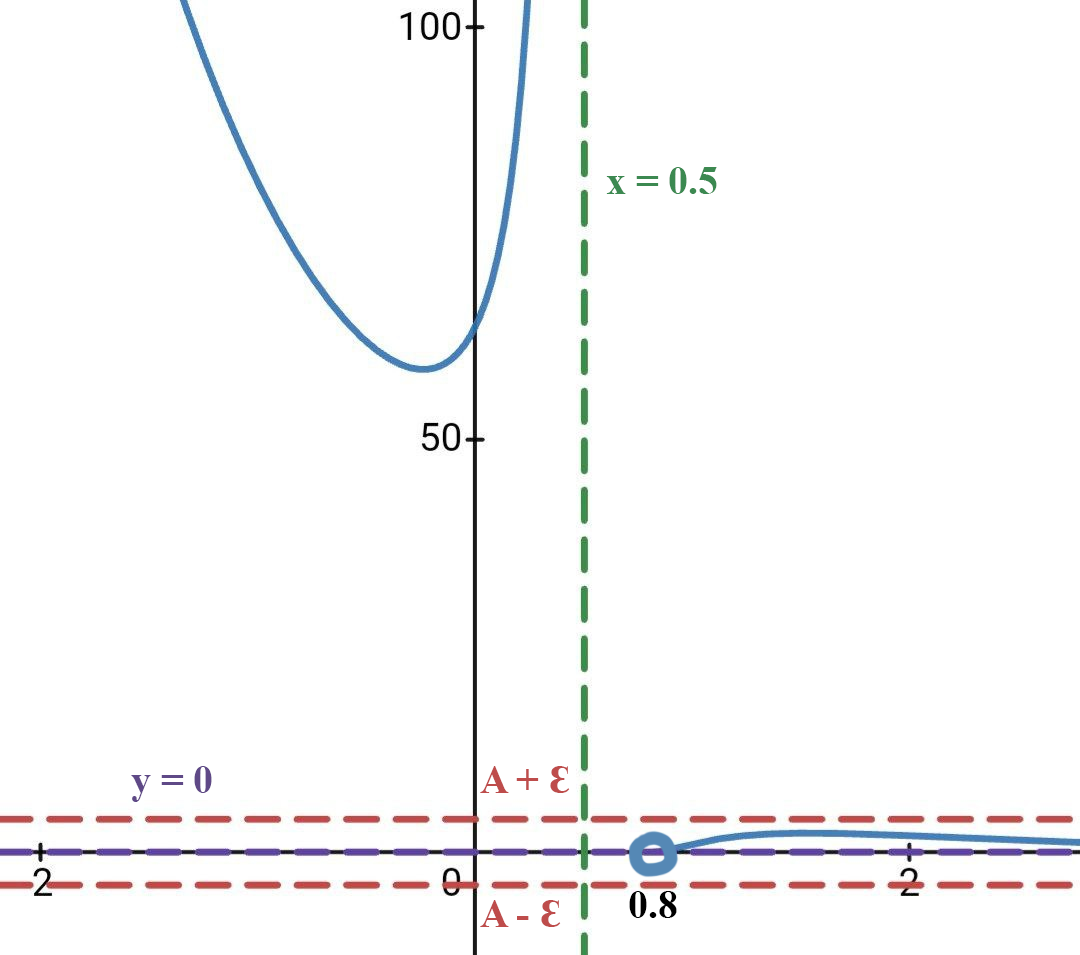
\includegraphics[height=200px]{graph.jpg} \\
На графике отсутствует $\delta$ окрестность, поскольку по определению предела функции на $\infty$ такой окрестности не существует \\
$x = 0.5, y = 0$ - асимптоты

% task 3
\newpage
    
    \section{\Large$f(x) = \frac{16x^2 - 9}{8x^2 - 18x + 9}, x_0 = \frac{3}{4}$}
    
\subsection{Вычисление предела}
$f(x) = \frac{16x^2 - 9}{8x^2 - 18x + 9}, x_0 = \frac{3}{4} $ \\ \\
Пусть $\lim\limits_{x \to x_0} f(x) = -4$ 

\subsection{Доказательство по Гейне}
\subsubsection{Определение предела функции в точке по Гейне}

\begin{equation*}
\begin{cases}
    $\forall \{x_n\} \subset D(f)$ \\
    $\forall n \geq N \in \mathbb{N} \ | \ x_n \neq x_0 \Rightarrow \lim\limits_{n \to \infty} f(x_n) = A$ \\
    $\lim\limits_{n \to \infty} x_n = x_0$ \\
\end{cases}
\end{equation*}

\subsubsection{План доказательства}
1. Напишем определение предела функции по Гейне \\
2. Предположим, что угаданный нами предел является таковым для $f(x)$ для $x_0$ \\
3. Нужно указать, что если предел $(1) \{f(x_n)\}_{n \to \infty}$ равен угаданному нами пределу, то $\forall \{x_n\} \to x_0$ и наоборот, посколько в определении по Гейне установлена связь между такими утверждениями \\
4. Для этого, используя определение предела последовательности через неравенство, выведем равносильнми преобразованиями из предела $(1)$ предел $(2)$, так же используя теорему о двух милиционерах (о сжатой переменной)

\subsubsection{Доказательство}
\begin{equation*}
\begin{cases}
    $\forall \{x_n\} \subset D(f)$ \\
    $\forall n \geq N \in \mathbb{N} \ | \ x_n \neq \frac{3}{4}$ \Rightarrow\\
    $\lim\limits_{n \to \infty} x_n = \frac{3}{4}$ \\
\end{cases}
\end{equation*}
$ \lim\limits_{n \to \infty} f(x_n) = -4 \iff \forall \varepsilon > 0 \ \exists N \in \mathbb{N} \ | \ \forall n \geq N \ | f(x_n) + n | < \varepsilon$ \\
При $n \to \infty$ разумно рассматривать малые $\varepsilon$, поэтому наложим на $\varepsilon$ ограничения: $\varepsilon \in (0; 1)$ (поскольку при $\varepsilon \geq 1$ определение предела последдовательности теряет смысл) \\ \\
$- \varepsilon < \frac{16x_n^2 - 9}{8x_n^2 - 18x_n + 9} + 4 < \varepsilon$ \\ \\
$- \varepsilon < \frac{12x_n - 9}{2x_n - 3} < \varepsilon$ \\ \\
Первая часть системы: \\ \\
$\frac{12x_n - 9}{2x_n - 3} < \varepsilon$ \\ \\
$6(\frac{x_n - 0.75}{x_n - 1.5}) < \varepsilon$ \\ \\
$\frac{x_n - 0.75}{x_n - 1.5} < \frac{\varepsilon}{6}$ (при $n \to \infty x_n \to \frac{3}{4} \Rightarrow (x_n - 1.5)$ при $n \geq N$ будет меньше нуля) \\ \\
$x_n - 0.75 > \frac{\varepsilon}{6}x_n - \frac{\varepsilon}{4}$ \\ \\
$(1 - \frac{\varepsilon}{6})x_n > 0.75 - \frac{\varepsilon}{4}$ \\ \\
$x_n > \frac{0.75 - \frac{\varepsilon}{4}}{1 - \frac{\varepsilon}{6}}$ \\ \\
Вторая часть системы: \\ \\
$\frac{12x_n - 9}{2x_n - 3} > - \varepsilon$ \\ \\
$6(\frac{x_n - 0.75}{x_n - 1.5}) > - \varepsilon$ \\ \\ 
$\frac{x_n - 0.75}{x_n - 1.5} > - \frac{\varepsilon}{6}$ (при $n \to \infty x_n \to \frac{3}{4} \Rightarrow (x_n - 1.5)$ при $n \geq N$ будет меньше нуля) \\ \\
$x_n - 0.75 < - \frac{\varepsilon}{6}x_n + \frac{\varepsilon}{4}$ \\ \\
$(1 + \frac{\varepsilon}{6})x_n < 0.75 + \frac{\varepsilon}{4}$ \\ \\
$x_n < \frac{0.75 + \frac{\varepsilon}{4}}{1 + \frac{\varepsilon}{6}}$ \\ \\
Возврат к системе: \\ \\
$\frac{0.75 - \frac{\varepsilon}{4}}{1 - \frac{\varepsilon}{6}} < x_n < \frac{0.75 + \frac{\varepsilon}{4}}{1 + \frac{\varepsilon}{6}}$ \\
Заметим, что при $n \to \infty \varepsilon \to 0$, тогда $\{\frac{0.75 - \frac{\varepsilon}{4}}{1 - \frac{\varepsilon}{6}}\} \to 0.75 -0$, а $\frac{0.75 + \frac{\varepsilon}{4}}{1 + \frac{\varepsilon}{6}} \to 0.75 +0$, таким образом по теореме о 2-х милиционерах (о сжатой переменной) \\
$\{x_n\}_{n \to \infty} \to 0.25$ \\
Поскольку все преобразования равносильны, то выполняется определение предела в точки по Гейне \\
Q.E.D.

\subsection{Иллюстрация}
Проиллюстрируем определение предела функции в точке по Гейне для $f(x)$ и подпоследовательности из $D(f) \{0.75 + \frac{1}{n}\}$ \\
$f(0.25 + \frac{1}{n}) = \frac{12n + 8}{-3n + 4}$ \\
Для $f(0.25 + \frac{1}{n})$ при $n \to \infty$ предел равен -4 \\
$\lim\limits_{n \to \infty} f(0.25 + \frac{1}{n} = \lim\limits_{n \to \infty} \frac{12n + 8}{-3n + 4} = - \lim\limits_{n \to \infty} \frac{12 - \frac{8}{n}}{3 - \frac{4}{n}} = -4$



% task 4
\newpage
    \section{В круг радиуса r вписан квадрат, в квадрат вписан круг, и так n раз. Найдите предел суммы площадей всех кругов и предел суммы площадей всех квадратов при $n \to \infty$}
\subsection{Графическая иллюстрация}
    \begin{tikzpicture}
    % main picture
    \draw (0,0) circle (2);
    \draw (-1.41,-1.41) rectangle (1.41,1.41);
    
    \draw (0,0) circle (1.41);
    \draw (-1,-1) rectangle (1,1);
    
    \draw (0,0) circle (1);
    \draw (-0.7,-0.7) rectangle (0.7,0.7);
    
    \draw (0,0) circle (0.7);
    \draw (-0.5,-0.5) rectangle (0.5,0.5);

    \draw (0,0) circle (0.5);
    \draw (-0.35,-0.35) rectangle (0.35,0.35);

    \draw (0,0) circle (0.35);
    \draw (-0.23,-0.23) rectangle (0.23,0.23);
    \draw (0,0) circle (0.23);

    % sub picture
    \draw (7,0) circle (2);
    \draw (5.59,-1.41) rectangle (8.41,1.41);
    \draw[-] (5.59,1.41) -- node[above] {$r\sqrt{2}$} (8.41,1.41);
    
    \draw (7,0) circle (1.41);

    \draw[-] (7,0) -- node[above] {r} (5.59,-1.41);
    \draw[-] (7,0) -- node[above] {r} (5.59,1.41);
    
    \end{tikzpicture}

\subsection{Математическая модель}
\subsubsection{Найдем зависимоть площадей}
    $S_{\textsubscript{круга1}} = \pi r_1^2$ \\ \\
    Сторона квадрата 1: \\
    $a_1 = 2(sin(\frac{\pi}{4}) r_1) = r_1\sqrt{2}$, тогда \\
    $S_{\textsubscript{квадр.1}} = 2r_1^2$ \\ \\
    Радиус круга 2: \\
    $r_2 = \frac{r_1\sqrt{2}}{2}$, тогда \\ 
    $S_{\textsubscript{круга2}} = \pi r_2^2 = \frac{\pi r_1^2}{2}$ \\ \\
    Сторона квадрата 2: \\
    $a_2 = 2(sin(\frac{\pi}{4}) r_2) = r_2\sqrt{2} = r_1$, тогда \\ \\
    $S_{\textsubscript{квадр.1}} = r_1^2$ \\ \\
    \ldots \\ \\
    Заметим зависимость площади квадрата от площади круга $S_{\textsubscript{квадр.}} = \frac{\pi}{2} S_{\textsubscript{круга}}$
\subsubsection{Основные формулы}  
    Есть круг радиуса r, для того чтобы найти его площадь воспользуемся формулой $S_{\textsubscript{круга1}} = \pi  r^2$ \\
    В него вписан квадрат, диагональ квадрата будет равна 2r, его сторона - $r\sqrt{2}$, тогда площадь квадрата найдём по формуле $S_{\textsubscript{квадр.1}} = 2r^2$ \\
    Радиус круга вписанного в квадрат будет $\frac{r\sqrt{2}}{2}$, тогда его площадь $S_{\textsubscript{круга2}} = \frac{\pi r^2}{2}$ \\
    Аналогиччо с площодью первого квадрата, найдем площадь второго по формуле $S_{\textsubscript{квадр.2}} = r^2$ \\
    И так далее для каждого из n кругов и квадратов, найдем их площади \\
    Для нахождения суммы площадей воспользуемся формулой суммы геометрической прогрессии - $S_n = \frac{b_1(q^n - 1)}{q- 1}$
  
\subsection{Аналитическое решение}

\subsubsection{Найдем суммарную площадь кругов}

    $S_1 = \pi  r^2$ \\ \\
    $S_2 = \frac{\pi r^2}{2}$ \\ \\
    $S_3 = \frac{\pi r^2}{4}$\\ \\
    $S_4 = \frac{\pi r^2}{8}$ \\ \\
    \ldots \\
    $S_n = \frac{\pi r^2}{2^n}$ \\ \\
    $S_{\textsubscript{общ.}} = \sum\limits_{i=1}^n S_i = \pi r^2 + \frac{\pi r^2}{2^{i-1}} + \ldots + \frac{\pi r^2}{2^{n-1}} = \pi r^2 \sum\limits_{i=1}^n \frac{1}{2^{i-1}}$ \\ \\
    $\frac{1}{2^{i-1}}$ является геометрической прогрессией, поэтому мы можем воспользоваться формулой суммы геометрической прогрессии, где 
    $q = \frac{1}{2}, b_1 = 1$: \\
    $\sum\limits_{i=1}^n \frac{1}{2^{i-1}} = \frac{\frac{1}{2^{n-1}} - 1}{\frac{1}{2} - 1}$ \\ \\
    Поскольку количество кругов стремится к $\infty$, верно следующее: \\
    $\lim\limits_{n \to \infty} \frac{\frac{1}{2^{n-1}} - 1}{\frac{1}{2} - 1} = \lim\limits_{n \to \infty} \frac{1 - \frac{1}{2^{n-1}}}{\frac{1}{2}} = 2$ \\ \\
    Тогда сумма площадей кругов $S_{\textsubscript{общ.}} = 2 \pi r^2$
    
    
\subsubsection{Найдем суммарную площадь квадратов}

    $S_{\textsubscript{квадр.}} = \frac{2}{\pi}S_{\textsubscript{круг}}$ (по 4.2.1), тогда \\ \\
    $S_1 = 2 r^2$ \\ \\
    $S_2 = \frac{2 r^2}{2}$ \\ \\
    $S_3 = \frac{2 r^2}{4}$\\ \\
    $S_4 = \frac{2 r^2}{8}$ \\ \\
    \ldots \\
    $S_n = \frac{2 r^2}{2^n}$ \\ \\
    $S_{\textsubscript{общ.}} = \sum\limits_{i=1}^n S_i = 2 r^2 + \frac{2 r^2}{2^{i-1}} + \ldots + \frac{2 r^2}{2^{n-1}} = 2 r^2 \sum\limits_{i=1}^n \frac{1}{2^{i-1}}$ \\ \\
    $\frac{1}{2^{i-1}}$ является геометрической прогрессией, поэтому мы можем воспользоваться формулой суммы геометрической прогрессии, где
    $q = \frac{1}{2}, b_1 = 1$: \\
    $\sum\limits_{i=1}^n \frac{1}{2^{i-1}} = \frac{\frac{1}{2^{n-1}} - 1}{\frac{1}{2} - 1}$ \\ \\
    Поскольку количество квадратов стремится к $\infty$, верно следующее: \\
    $\lim\limits_{n \to \infty} \frac{\frac{1}{2^{n-1}} - 1}{\frac{1}{2} - 1} = \lim\limits_{n \to \infty} \frac{1 - \frac{1}{2^{n-1}}}{\frac{1}{2}} = 2$ \\ \\
    Тогда сумма площадей квадратов $S_{\textsubscript{общ.}} = 4 r^2$

\subsubsection{Общая площадь}

    Имея сумму площадей кругов $S_{\textsubscript{круг.общ.}} = 2 \pi r^2$ и сумму площадей квадратов $S_{\textsubscript{квадр.общ.}} = 4 r^2$, найдем общую сумму площадей фигур \\
    $S_{\textsubscript{общ.}} = 2 \pi r^2 + 4 r^2 = 2 r^2 (\pi + 2)$
    


    
% evaluation paper
\newpage
\[
\renewcommand{\arraystretch}{2}
\begin{tabular}{| c | c |}
 \hline
    \hugeУчастник & \hugeВклад в \% \\
 \hline
    \hugeКаренин Константин & \huge33.(3) \\
 \hline
    \hugeГонин Сергей & \huge33.(3) \\
 \hline
    \hugeТемиров Тимур & \huge33.(3) \\
 \hline
\end{tabular}
\]
\end{document}